
\documentclass[12pt,a4paper,oneside]{book}
\usepackage[utf8]{inputenc}
\usepackage{graphicx} %input gambar
\usepackage{amsmath}
\usepackage{amsfonts}
\usepackage{amssymb}
%
\usepackage{mathptmx}
\usepackage[T1]{fontenc}

% Garis tepi (margin)
\usepackage{geometry}
 \geometry{
 left=4cm,
 top=4cm,
 right=3cm,
 bottom=3cm,
 }

% mengatur 1 cm baris pertama paragraf
\usepackage{indentfirst}
\setlength{\parindent}{1cm}

% Mengkompres cite
\usepackage[numbers]{natbib}

% Mengatur header dan foother
\usepackage{fancyhdr}
\pagestyle{fancy}
\fancyhead[L]{}  %mengosongkan head kiri
\fancyhead[R]{\thepage}  %memberi nomor page head kanan
\renewcommand{\headrulewidth}{0pt} %menghilangkan garis
\fancyfoot{} % menghilangkan footer

% change name Daftar Isi, Daftar Pustaka jadi section
\renewcommand{\contentsname}{DAFTAR ISI}
\renewcommand{\bibsection}{\section{Daftar Pustaka}}

% change languange dan pemenggalan kata
\usepackage[indonesian]{babel}
\sloppy

% numbering on section
\renewcommand\thesection{\Alph{section}.}
\renewcommand\thesubsection{\thesection\arabic{subsection}}

% baris antar paragraf
\linespread{1.5}

% mengatur title section
\usepackage{titlesec}
\titleformat{\chapter}[display]   
{\centering\normalfont\large\bfseries}{\chaptertitlename\ \thechapter}{0pt}{\large}   
\titlespacing*{\chapter}{0pt}{-50pt}{40pt}

% untuk modif numbering
\usepackage{enumitem}


\begin{document}

\begin{titlepage}
   \begin{center}

       \textbf{PENERAPAN \textit{K-MEANS} DAN ALGORITMA GENETIKA UNTUK MENYELESAIKAN MTSP}
       
       %\vspace{1.5cm}
       \vfill
       
       \textbf{PROPOSAL SKRIPSI}
       
       %\vspace{1.5cm}
       \vfill
       
       
\includegraphics[width=0.4\textwidth]{logo.png}
       
       %\vspace{1.5cm}
       \vfill
       
       \textbf{OLEH:}
       
       \vspace{0.5cm}

       \textbf{\underline{MUHAMMAD FAIZ NAILUN NI'AM}}
       
       NIM : 1842200034

       \vfill
       
       UNIVERSITAS NURUL JADID\\
       PAITON PROBOLINGGO\\
       \textbf{FAKULTAS SOSIAL DAN HUMANIORA}\\
       PROGRAM STUDI PENDIDIKAN MATEMATIKA
       
       \vspace{0.5cm}
       
       2021       
   
   \end{center}
\end{titlepage}

% Halaman daftar isi
\newpage
\frontmatter
\tableofcontents

% Halaman isi
\newpage
\mainmatter
% Hasil revisi ibu shofia

\section{Latar Belakang Masalah}

Kabupaten Probobolinggo adalah salah satu dari beberapa kabupaten yang sedang berkembang di provinsi Jawa Timur. Banyak sekolah-sekolah menengah yang tersebar di Kabupaten Probolinggo. Oleh karena itu jika sebuah lembaga pendidikan yang sedang mengadakan kegiatan di Kabupaten Probolinggo dan ingin menyebarkan pamflet atau undangan diperlukanlah sebuah rute yang paling dekat agar dapat mempermudah perjalanan.

Selama bertahun-tahun, telah banyak penelitian tentang \textit{Multiple Traveling Salesman Problem} (MTSP). Berbagai metode telah digunakan untuk mencari solusi MTSP, salah satunya adalah Algoritma Genetika (AG), ada banyak upaya untuk menggunakan AG dalam pengklasteran, metode ini menemukan solusi lebih cepat daripada beberapa algoritma lain yang digunakan untuk pengklasteran \cite{krishna1999genetic}. Kemampuan menemukan solusi dari AG dimanfaatkan untuk mencari pusat klaster yang sesuai di ruang fitur sedemikian rupa sehingga kesamaan dari klaster yang dihasilkan dioptimalkan \cite{maii2000genetic}. Ada juga upaya untuk menggunakan metode paralel untuk TSP untuk meningkatkan efisiensi \cite{li2016parallel}. Namun, menurut Zhang efisiensi AG akan menurun dengan cepat jika digunakan pada skala kota besar \cite{zhang2014parallel}. 

Penggunaan AG dan dan algoritma \textit{k}-means adalah metode yang efektif untuk menyelesaikan MTSP, selain itu juga dapat menghindari persilangan antar salesman seperti yang dibahas oleh Lu pada artikelnya \cite{inproceedings}. Dari gabungan semua perspektif tersebut, dalam proposal ini, digunakanlah AG dan \textit{k}-means untuk menyelesaikan kasus pembagian klaster dan pencarian rute terdekat tiap klaster di seluruh SMP di Kabupaten Probolinggo.

\section{Identifikasi Masalah}

Dari latar belakang yang telah diuraikan,
identifikasi masalahnya adalah sebagai berikut.
\begin{enumerate}
	\item Penggunaan $k$-means dan algoritma genetika untuk mencari solusi MTSP.
	\item Perbandingan mencari solusi MTSP dengan menggunakan $k$-means dan Algoritma Genetika dibandingkan dengan menggunakan Algoritma Genetika tanpa menggunakan $k$-means.
\end{enumerate}

\section{Rumusan Masalah}

Berdasarkan identifikasi masalah maka rumusan masalah yang akan dibahas dalam penelitian ini yaitu:
\begin{enumerate}
    \item Bagaimana cara mencari solusi \textit{multiple traveling salesman problem} dengan $k$-means dan algoritma genetika?
    \item Bagaimana perbandingan mencari solusi MTSP dengan menggunakan $k$-means dan Algoritma Genetika dibandingkan dengan menggunakan Algoritma Genetika tanpa menggunakan $k$-means?
\end{enumerate}

\section{Tujuan Penelitian}

Berdasarkan rumusan masalah di atas, tujuan dari penelitian ini yaitu untuk:
\begin{enumerate}
	\item Mengetahui cara menemukan solusi \textit{multiple traveling salesman problem} dengan \textit{k-means} dan algoritma genetika.
	\item Mengetahui perbandingan mencari solusi MTSP dengan menggunakan \textit{k-means} dan Algoritma Genetika dibandingkan dengan menggunakan Algoritma Genetika tanpa menggunakan \textit{k-means}?
\end{enumerate}


% sudah direvisi ibu shofia

\section{Manfaat Penelitian}

Manfaat dari penelitian ini yaitu:
\begin{enumerate}
	\item Bagi Penulis, mengetahui cara menyelesaikan kasus \textit{Multiple Traveling Salesman Problem} yang telah dikembangkan yaitu dengan menggunakan metode $K$-Means \textit{Clustering} dan Algoritma Genetika serta penulis dapat mengembangkan ilmu pemorgraman python pada komputer.

	\item Bagi Program Studi Pendidikan Matematika, menambah ilmu mengenai metode optimasi dan pencarian rute terdekat yang dapat diterapkan serta dipelajari kembali oleh mahasiswa pendidikan matematika untuk tahun-tahun selanjutnya
	
	\item Bagi Masyarakat, dapat menggunakan metode tersebut untuk menyelesaikan kasus \textit{Multiple Traveling Salesman Problem}, seperti penyebaran pestisida, pengintaian musuh pada militer, pendistribusian barang, dan lain-lain.
	
\end{enumerate}


\section{Definisi Konsep}

Dalam proposal ini, membahas tentang \textit{Multiple Traveling Salesman Problem} yang merupakan perluasan dari \textit{Travelling Salesman Problem} (TSP). TSP adalah permasalahan pencarian rute terpendek seorang salesman dari suatu kota ke kota lain tepat satu kali dan kembali ke kota yang sama. Sedangkan MTSP adalah permasalahan TSP oleh beberapa orang salesman dengan tujuan yang sudah dibagi.

Algoritma yang digunakan untuk membagi adalah $K$-means. $K$-means adalah jenis metode klasifikasi yang membagi item data menjadi beberapa klaster. Algoritma Genetika (AG) digunakan untuk pencarian rute terpendek. AG adalah algoritma yang digunakan untuk mencari solusi dari permasalahan dengan cara yang terispirasi dari teori evolusi. Dalam hal ini, algoritma genetika dapat juga digunakan untuk pencarian sebuah rute terpendek dalam sebuah kasus perjalanan. Untuk mengukur jarak antar 2 titik yang digunakan adalah metode euclidean distance.


% sudah direvisi ibu shofia

\section{Penelitian Terdahulu}

Ada beberapa hasil penelitian sebelumnya yang memiliki keterkaitan dengan penelitian ini. Penelitian berjudul "Applying K-means and Genetic Algorithm for Solving MTSP" \cite{inproceedings}. Penelitian tersebut membahas tentang persilangan jalur antar tiap salesman yang dapat dihindari dengan menggukan Algoritma Genetika dan \textit{K}-means.

Penelitian kedua berjudul "Optimasi \textit{Multiple Travelling Salesman Problem} (M-TSP) Pada Penentuan Rute Optimal Penjemputan Penumpang \textit{Travel} Menggunakan Algoritme Genetika" \cite{raditya2017optimasi}. Penelitian tersebut membahas tentang permasalahan MTSP yaitu beberapa orang salesman yang akan berangkat dari kantor \textit{travel} menuju ke alamat penjemputan masing-masing penumpang. Pada permasalahan tersebut menggunakan representasi permutasi, proses reproduksi \textit{crossover} dengan \textit{one cut point crossover}, proses mutasi dengan \textit{exchange mutation}, dan proses seleksi dengan \textit{elitism selection}.

Mayuliana, N. K., Kencana, E. N., dan Harini, L. P. I. dalam artikelnya yang berjudul “Penyelesaian Multitraveling Salesman Problem dengan Algoritma Genetika” \cite{mayuliana2015penyelesaian}, mempelajari tentang kinerja algoritma genetika berdasarkan jarak minimum dan waktu pemrosesan yang diperlukan untuk 10 kali pengulangan untuk setiap kombinasi kota penjual. Artikel karangan Al-Khateeb, B., dan Yousif, M. berjudul "\textit{SOLVING MULTIPLE TRAVELING SALESMAN PROBLEM BY MEERKAT SWARM OPTIMIZATION ALGORITHM}" \cite{al2019solving} dalam artikel ini mengusulkan algoritma metaheuristik yang disebut algoritma \textit{Meerkat Swarm Optimization} (MSO) untuk memecahkan MTSP dan menjamin solusi berkualitas baik dalam waktu yang wajar untuk masalah kehidupan nyata.


% sudah direvisi ibu shofia

\section{Kajian Pustaka}

\subsection{\textit{Multiple Traveling Salesman Problem}}

Menurut Al-Omeer dan Ahmed, \textit{Multiple Travelling Salesman Problem} (MTSP) adalah salah satu kombinatorial optimasi masalah, yang dapat didefinisikan sebagai berikut: Ada $m$ jumlah salesman yang harus melakukan perjalanan ke $n$ sejumlah kota dimulai dengan depot dan berakhir di depot yang sama \cite{al2019comparative}. Selanjutnya para salesman harus melakukan perjalanan dari satu kota ke kota lain secara terus menerus tanpa mengulang kota mana saja yang telah dilintasi oleh para salesman dan mempertimbangkan jalur terpendek selama perjalanan tersebut. Metode MTSP sebenarnya banyak sekali, namun yang digunakan dalam penelitian ini adalah algoritma genetika dan algoritma \textit{k}-means.

Contoh solusi MTSP:

\begin{figure}[h!]
  \centering
  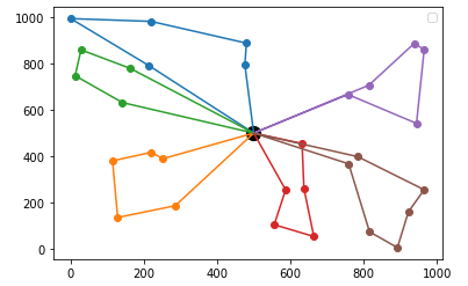
\includegraphics[width=0.5\textwidth]{Picture1.png}
  \caption{Solusi MTSP dengan membagi menjadi 6 klaster}
\end{figure}

\begin{figure}[h!]
  \centering
  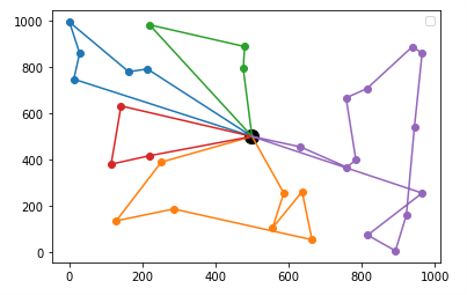
\includegraphics[width=0.5\textwidth]{Picture2.png}
  \caption{Solusi MTSP dengan membagi menjadi 5 klaster}
\end{figure}

\subsection{Algoritma}

Maulana menyebutkan dalam artikelnya algoritma adalah kumpulan perintah untuk menyelesaikan suatu masalah dan diselesaikan dengan cara sistematis, terstruktur dan logis \cite{maulana2017pembelajaran}. Algoritma digunakan untuk memcahkan permasalahan yang dialami oleh seorang pengguna program.

\subsection{Algoritma $k$-means}

$K$-Means adalah jenis metode klasifikasi tanpa pengawasan yang mempartisi item data menjadi satu atau lebih klaster \cite{agusta2007k}. $K$-Means mencoba untuk memodelkan suatu dataset ke dalam klaster-klaster sehingga item-item data dalam suatu klaster memiliki karakteristik yang sama dan memiliki karakteristik yang berbeda dengan cluster lainnya.

Menurut S Monalisa \cite{monalisa2018klasterisasi} tahapan mengklaster menggunakan algoritma \textit{k}-means adalah sebagai berikut:

\begin{enumerate}
	\item Menentukan banyak klaster sesuai dengan keinginan
	\item Pilih beberapa \textit{centroid} secara acak sesuai banyak klaster
	\item Hitung jarak titik ke centroid dengan rumus \textit{euclidean distance}
	\begin{equation}
	d_{xy}=\sqrt{\sum_{i=1}^{n}(x_i-y_i)^{2}}
	\end{equation}
	\item Titik-titik yang tersebar masuk ke klaster yang sama dengan titik \textit{centroid} yang paling dekat
	\item Perbarui \textit{centroid} dengan menghitung nilai rata-rata nilai pada masing-masing klaster
	\item Lakukan iterasi sebanyak mungkin dengan kembali ke tahapan 3 sampai tidak ada perubahan klaster atau perubahan nilai \textit{centroid}
\end{enumerate}

\subsection{Algoritma Genetika}

Pada artikel Hermanto disebutkan bahwa algoritma genetika adalah algoritma yang digunakan untuk mencari solusi suatu permasalahan dengan cara yang lebih alami yang terispirasi dari teori evolusi  \cite{hermawanto2003algoritma}. Dalam hal ini, algoritma genetika dapat juga digunakan untuk pencarian sebuah rute terpendek dalam sebuah kasus perjalanan.

Menurut Armanda RS \cite{armanda2016penerapan} dalam artikelnya menyampaikan penyelesaian masalah menggunakan algoritma genetika memerlukan beberapa tahapan sebagai berikut:

\begin{enumerate}
	\item Menyiapkan populasi, dalam penelitian ini yang digunakan adalah data yang telah diklaster menggunakan algoritma \textit{k}-means
	\item Melakukan reproduksi dengan crosover dan mutasi pada pembentukan awal populasi
	\item Seleksi dengan metode elitism
	\item Menentukan nilai fitness agar mendapatkan solusi akhir yang optimal. Berikut merupakan persamaan perhitungan dalam mengetahui nilai fitness pada metode algoritma genetika
	\begin{equation}
	fitness=\frac{10000}{RMSE}
	\end{equation}
	\item Iterasi dilakukan untuk generasi berikutnya.
\end{enumerate}

\section{Metode Penelitian}

Metode penelitian dalam proposal ini adalah metode penelitian dan pengembangan. Melalui metode ini diharapkan dapat mengembangkan algoritma yang diteliti.

Langkah-langkah yang akan dilakukan dalam penelitian:
\begin{enumerate}
	\item Menggunakan bahasa pemrograman \textit{Python} untuk mempermudah pengerjaan.
	
	\item Menyiapkan dataset random menggunakan "\textbackslash import random" pada \textit{Python} yang akan digunakan sebagai uji coba.
	
	\item Membagi titik pada MTSP menggunakan Algoritma $K$-Means menjadi $m$ klaster sesuai dengan distribusinya.
	
	\item Menggunakan Algoritma Genetika untuk menemukan rute terpendek untuk masing-masing klaster.
	
	\item Membandingkan penyelesaian MTSP dengan menggunakan algoritma genetika dan $k$-means dibandingkan dengan algoritma genetika tanpa $k$-means
	
	\item Menganalisi dan mengevaluasi data yang dihasilkan

\end{enumerate}

\section{Sistematika Penelitian}

Agar penulisan dalam penelitian yang diusulkan lebih terarah,
maka diperlukan sistematika penelitian.
Terkait hal tersebut,
sistematika penulisan dalam penelitian yang dilakukan nantinya adalah sebagai berikut.

\begin{enumerate}[label=]

	\item BAB I PENDAHULUAN 
	\begin{enumerate}[label=\Alph*.]
		\item Latar Belakang Masalah
		\item Rumusan Masalah
		\item Manfaat penelitian
		\item Tujuan Penelitian dan Pengembangan
		\item Batasan Masalah Penelitian
	\end{enumerate}

	\item BAB II KAJIAN PUSTAKA 
	\begin{enumerate}[label=\Alph*.]
		\item Penelitian relevan
		\item Dasar Teori
	\end{enumerate}

	\item BAB III KERANGKA TEORITIK DAN PENGEMBANGAN 
	\begin{enumerate}[label=\Alph*.]
		\item Model Penelitian dan Pengembangan
		\item Prosedur Penelitian dan Pengembangan
	\end{enumerate}

	\item BAB IV HASIL 
	\begin{enumerate}[label=\Alph*.]
		\item Penyajian Data Uji Coba
		\item Analisis Data
		\item Revisi Produk
	\end{enumerate}

	\item BAB V PENUTUP 
	\begin{enumerate}[label=\Alph*.]
		\item Kesimpulan
		\item Saran
	\end{enumerate}

\end{enumerate}


%penelitian akan mempu menghasilkan suatu produk yang memiliki nilai validasi tinggi, karena melalui serangkaian uji coba di lapangan dan divalidasi. Sistematika penelitian ini dibagi menjadi 4 tahap:
%
%\begin{enumerate}
%
%	\item Perencanaan
%	
%	Kegiatan yang dilakukan dalam tahap ini adalah sebagai berikut: penyusunan rancangan penelitian, penyiapan alat-alat penelitian, penetapan data penelitian, menyusun instrumen penelitian.
%	
%	\item Pelaksanaan
%	
%	Pada tahap ini peneliti selain pelaksana penelitian  juga mencari informasi data, yaitu membaca artikel penelitian sebelumnya yang berkaitan. Selain itu peneliti juga menyiapkan aplikasi yang akan digunakan untuk membantu perhitungan.
%	
%	\item Analisis Data
%	
%	Analisis data dilakukan setelah peneliti melakukan beberapa uji coba pada beberapa sampel data.
%	
%	\item Evaluasi Semua Data
%	
%	Data yang telah dianalisis kemudian dievaluasi sehingga diketahui bahwa metode ini merupakan metode yang efektif untuk menyelesaikan \textit{Multiple Traveling Salesman Problem} (MTSP).

%\end{enumerate}

% Daftar Pustaka
\bibliographystyle{vancouver}
\bibliography{library}


\end{document}